\section{Description of the Characterization Problems}
\label{sec:AngleProbDesc}

In characterizing the $\Omega$ methods, we aim to determine in which problems
the $\Omega$-methods perform well, and then quantify that success.
First, it must be determined how effective the
$\Omega$-methods are in reducing the variance for a tally result in Monte Carlo.
This will be done by assessing and comparing the FOMs between different VR methods.
Also, the method should be investigated on a diverse set of anisotropic
problems. By constructing problems that have
different mechanisms by which the flux may be or become
anisotropic, potential strengths or weaknesses of the method can be identified.
Another desirable metric would be to quantify the method's success given the
degree of anisotropy in the problem. Recall that different
means of quantifying the flux
anisotropy were presented in Section \ref{sec:anisotropy_quant}. With a diverse
selection of characterization problems, we will obtain variation in the flux
anisotropy in each problem as well as the resultant FOMs. This will provide us
with a path forward with which to use the $\Omega$-methods in a deeper
angular-sensitivity study, which will be discussed in Section
\ref{sec:DetAngle}.

\subsection{Identification of Anisotropy-Inducing Physics}
\label{subsec:AngleProbID}

There exists a rich history of using hybrid methods in problems with strong
angular dependence, as summarized in Chapter \ref{sec:lit_review}. Angular
dependence may appear in a problem by way of several means.
Mosher et al. noted in their threat-detection work with ADVANTG
that problems with strongly directional sources and
problems with ``thin'' materials like air were difficult for ADVANTG to effectively
reduce the variance. The attributed this to strongly anisotropic behavior of the
importance function that were not reflected well by the scalar flux
\cite{mosher_automated_2009}. Sweezy also found that weight windows obtained
from a hybrid S$_N$ calculation were not good for a dogleg void problem,
where ray effects from the $S_N$ calculation generated poorer weight windows
than a method without ray effects \cite{sweezy_automated_2005}.
In their work with angular-CADIS, Peplow et
al. also found that CADIS struggled with thin material streaming in a spherical
boat test problem \cite{peplow_consistent_2012}.

The examples of angle-dependence in problems affecting hybrid methods' success
illustrate that the flux can have anisotropy resulting from more than one
mechanism. Based on these examples, we have identified several separate
processes that affect the flux anisotropy. These processes can be grouped into
three categories: anisotropy in the flux resulting from a strongly
directional source; anisotropy resulting from strong differences between
material properties (this can be due to differences in
materials spatially and due to cross section); and anisotropy in the flux
from algorithmic limitations (ray effects).

[From the problems that didn't work for other methods, extrapolate and describe
the physical reasons why these problems caused issues.]

[Make sure to talk about both physical effects and deterministically-introduced
issues, like ray effects.]

It is important to note that these broad categories of anisotropy-inducing
physics are targeted towards \textit{realistic} occurrences of anisotropies in
the flux. There are also computational effects that influence flux anisotropy,
namely ray effects. Ray effects are common in situations where there are strong
streaming effects. As describe in Sections \ref{sec:contributon} and
\ref{sec:applicationprobs}, ray effects occur when particles have long mean free
paths and are an effect from the angular discretization $S_N$ transport. As a
result, anisotropies in the flux arising from ray effects may also affect the
ability of the $\Omega$ methods to effectively reduce tally variances.

In this subsection, four primary physical mechanisms by which the flux may
be anisotropic were identified. These are streaming paths, problems with high
scattering effects, problems with high material heterogeneity (specifically with
materials with strong differences in scattering and absorption probabilities),
and problems with monodirectional sources. As described in the preceding
paragraphs, a few of these mechanisms may overlap
with one another. They comprise a large subset of flux
anisotropy-inducing physics, and combined with different geometric arrangements
in sample problems a diverse group anisotropic problems can be formulated. These
problems can then be used to characterize the $\Omega$-methods.

\subsection{Problem Specifications}
\label{subsec:ProbSpecs}

With the anisotropy-inducing physics described in Section
\ref{subsec:AngleProbID}, a set of characterization problems that have
different combinations of each of these effects can be conceptualized. With
different anisotropy-inducing physics in the system, these problems will provide
an overview of how the $\Omega$-methods perform in an assortment of anisotropic
problems. The primary anisotropy-inducing features identified are: streaming
paths, material heterogeneity, materials with highly differing scattering
probabilities, and monodirectional sources. As previously described, these fall
into two broad categories: anisotropy caused by the problem materials and
geometry, and anisotropy caused by the source definition. In the next few
paragraphs, each problem will be described and will be accompanied by
a justification for which
anisotropy-inducing physics is in each problem. A summary of which physics are
in each problem is provided in Table \ref{tab:probphysics}.

\subsubsection*{Experimental Beamline}

\begin{figure}[h!]
  \centering
  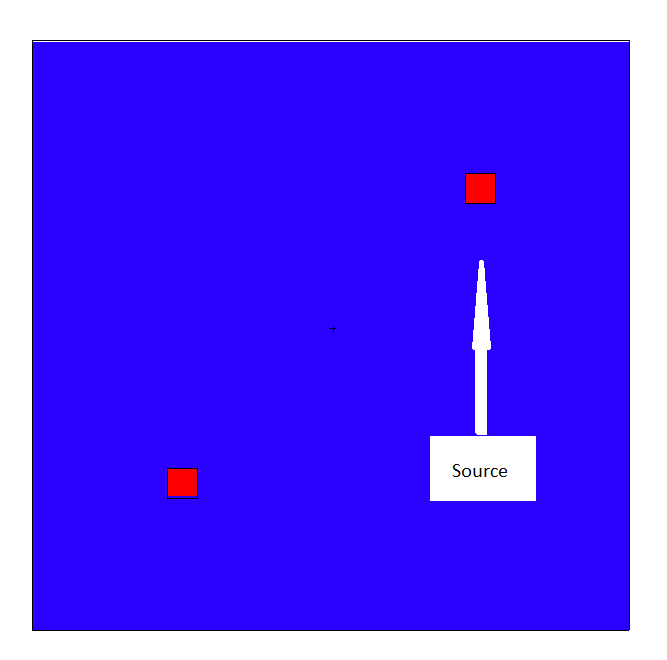
\includegraphics[height=8cm]{./chapters/characterization_probs/figures/geometries/beam.png}
  \caption[Nuclear physics experimental beamline.]{Nuclear physics experimental beamline.}
  \label{fig:beamgeom}
\end{figure}

The experimental beamline illustrated in Fig. \ref{fig:beamgeom} is an
application problem that will have strong angular dependence in the flux. The
facility is primarily air, with two sodium iodine detectors in the room. The
beamline--a monodirectional source--is aimed towards the first detector, and
the response in the second detector (at a 45\degree angle
relative to the beamline) is to be optimized with CADIS. In this problem, we
expect anisotropy to occur in the flux from both the monodirectional source and
the very strong streaming effects that will occur from the low-density air. This
problem will also be very high energy, with little opportunity for particles to
slow down from moderating materials. The only moderating materials in the
problem are located in the detectors. As a result, this problem will have a
significant amount of leakage out of the vacuum boundary conditions.

\subsubsection*{Maze Variants}

\begin{figure}[h!]
  \centering
  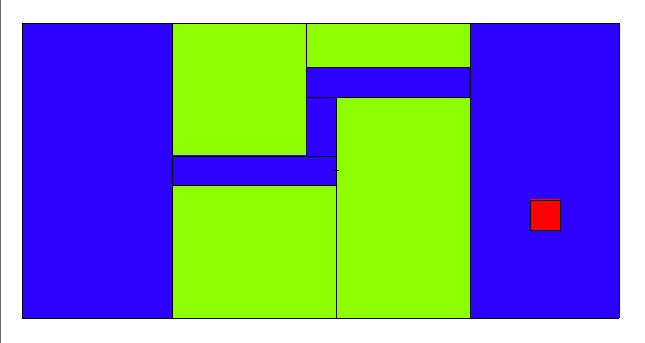
\includegraphics[width=10cm]{./chapters/characterization_probs/figures/geometries/maze2.png}
  \caption[Single turn labyrinth geometry.]{Single turn labyrinth geometry.}
  \label{fig:maze2geom}
\end{figure}

\begin{figure}[h!]
  \centering
  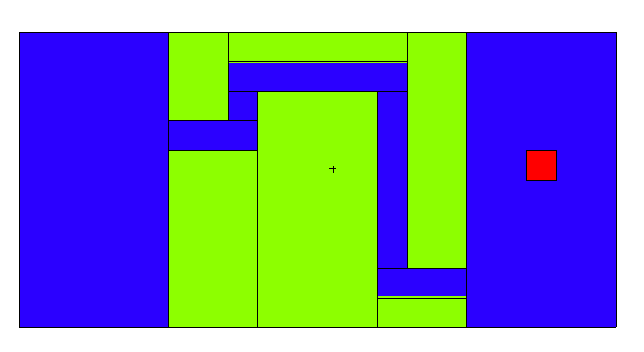
\includegraphics[width=10cm]{./chapters/characterization_probs/figures/geometries/maze1.png}
  \caption[Multi-turn labyrinth geometry.]{Multi-turn labyrinth geometry.}
  \label{fig:maze1geom}
\end{figure}

\subsubsection*{Steel beam in Concrete}

\begin{figure}[h!]
  \centering
  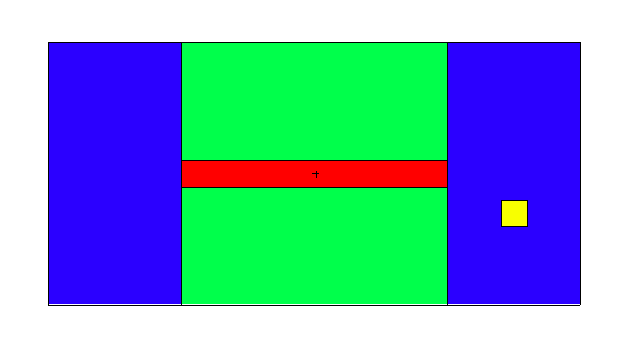
\includegraphics[width=12cm]{./chapters/characterization_probs/figures/geometries/prob-1.png}
  \caption[Steel plate embedded in concrete.]{Steel plate embedded in concrete.}
  \label{fig:prob1geom}
\end{figure}

\subsubsection*{U-shaped corridor}

\begin{figure}[h!]
  \centering
  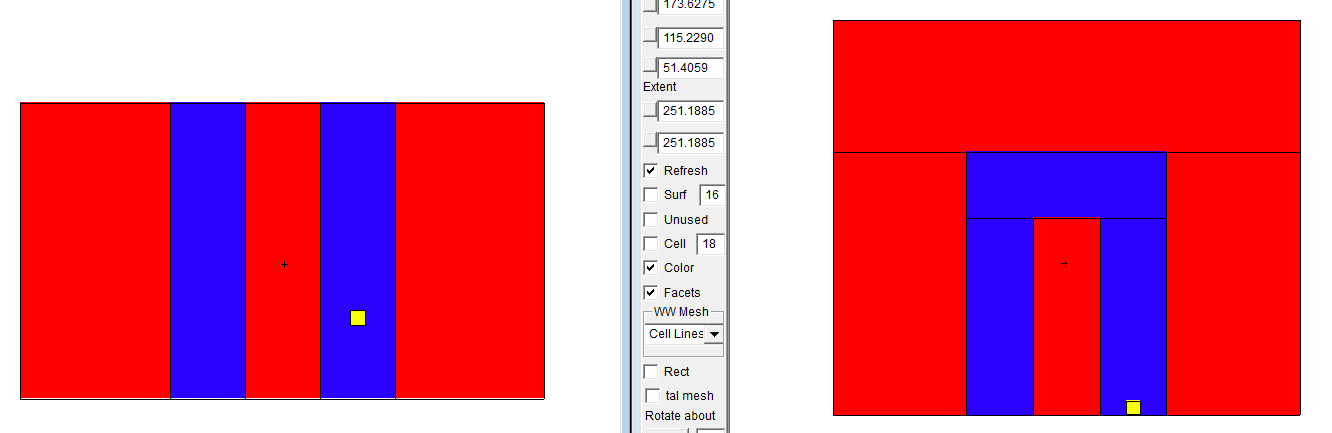
\includegraphics[width=15cm]{./chapters/characterization_probs/figures/geometries/prob-2.png}
  \caption[U-shaped corridor in concrete]{U-shaped corridor in concrete.}
  \label{fig:prob2geom}
\end{figure}

\subsubsection*{Concrete shielding with rebar}

\begin{figure}[h!]
  \centering
  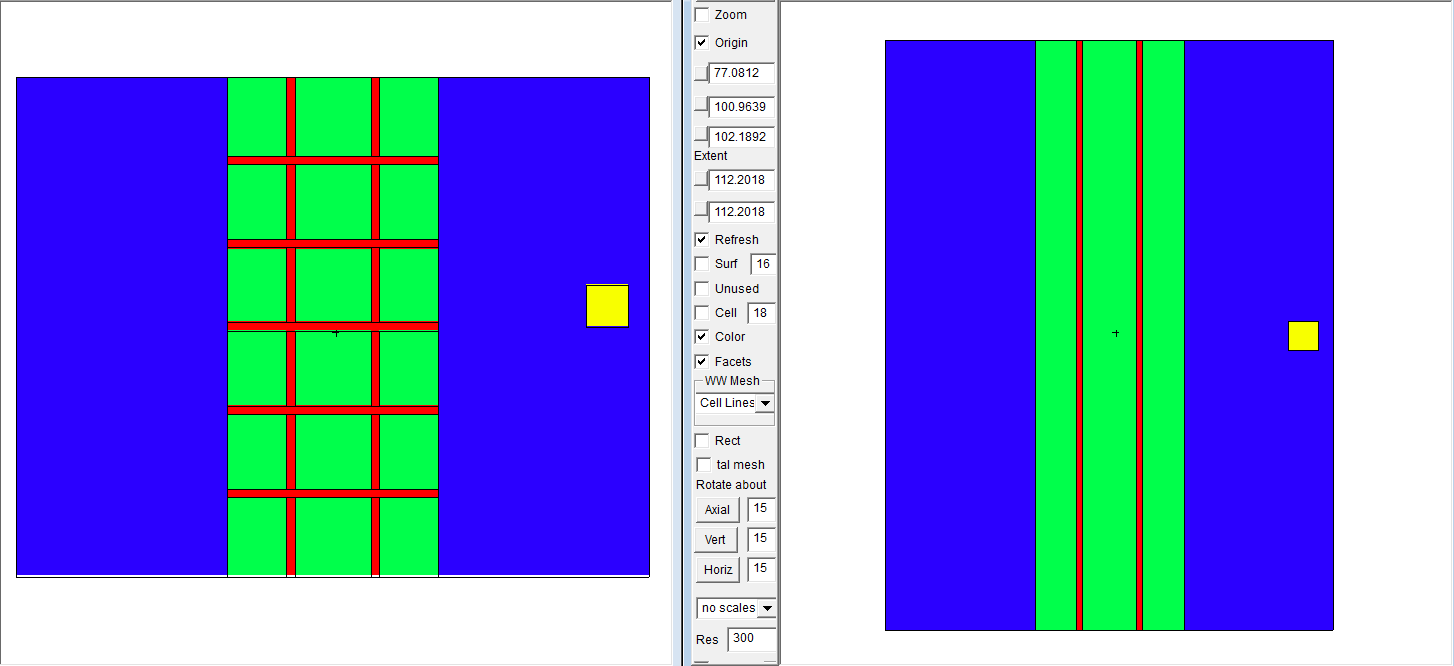
\includegraphics[width=15cm]{./chapters/characterization_probs/figures/geometries/prob-4.png}
  \caption[Concrete shielding with rebar]{Concrete shielding with rebar.}
  \label{fig:prob4geom}
\end{figure}

\subsubsection*{Nuclear medicine therapy room}

\begin{figure}[h!]
  \centering
  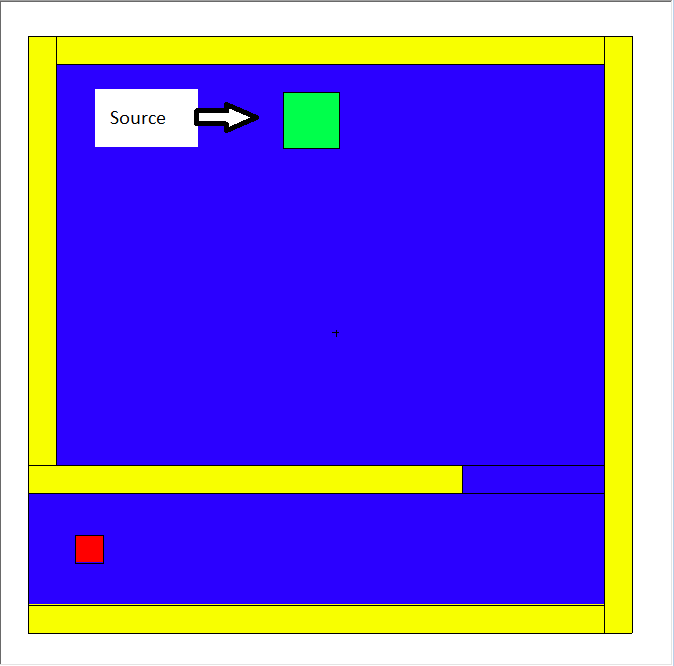
\includegraphics[height=8cm]{./chapters/characterization_probs/figures/geometries/therapy-room.png}
  \caption[Nuclear medicine therapy room.]{Therapy room geometry.}
  \label{fig:therapygeom}
\end{figure}

Now that the broad subset of characterization problems have been described,
the physics that each contains is summarized in Table \ref{tab:probphysics}.
Upon glancing at the table, one may see that it can be difficult to separate
out one physical mechanism from another when constructing problems. This is a
deficiency of the characterization problem construction, and is certainly an
area that may be improved upon in future work.

\begin{table}[h!]
  \centering
  \begin{tabular}{l|C{2cm}C{2cm}C{2cm}C{2cm}C{2cm}}
% \begin{tabular}{l|ccccc}
\toprule
\multirow{2}{*}{Problem Name} &  \multicolumn{4}{c}{Problem Coverage} \\
{} &  Streaming Paths & Highly Scattering & Material Heterogeneity &
Monodirectional Source & Ray \newline Effects \\
\midrule
Beamline              & x &   &   & x & x \\
Maze variants         &   &   &   &   &   \\
\textit{Single turn}  & x & x & x &   & x \\
\textit{Multi-turn}   & x & x & x &   & x \\
Steel plate           &   & x & x & x & x$^{\dagger}$  \\
U-shaped corridor     & x & x & x &   &   \\
Shielding with rebar  &   & x & x & x &   \\
Therapy Room          & x &   & x & x & x \\
\bottomrule
\end{tabular}
\begin{flushleft}
\footnotesize{
  $^{\dagger}$ May have ray effects in low density region exiting the metal
  plate, but effects will be less pronounced than other problems.
}
\end{flushleft}

  \caption[Anisotropy-inducing physics of each of the characterization problems.]
  {Anisotropy-inducing physics of each of the characterization problems.
  Each identified anisotropy-inducing physical metric is used in different
  combinations for the characterization problems. This will help to aid in
  extrapolating to which real problems the $\Omega$-methods may be applied.}
  \label{tab:probphysics}
\end{table}
